\chapter{Analisi e conclusioni}
Il testing del progetto sulla scheda Nexys4 DDR è stato condotto
attraverso la porta seriale della scheda e mediante l'uso di uno
script Python che automatizzasse la riproduzione di un file MIDI 
(si veda \code{scripts/play\_midi\_file.py}.
Per effettuare il testing funzionale delle varie componenti del progetto
si è fatto uso di \textit{testbenches} scritti in VHDL, che fornissero
un input prefissato a un certo componente per verificarne la risposta,
utilizzando sempre GHDL.
In particolare il testbench descritto nel file
 \code{vhdl/mono\_synth\_engine\_tb.vhd} provvede a testare l'intera
architettura riproducendo una singola nota.
L'uscita del blocco \code{pwm\_encoder} viene quindi salvata ad ogni
ciclo di clock su un file txt, che viene in seguito processato
dallo script \code{scripts/plot\_pwm\_output.py} che lo filtra
digitalmente e visualizza il segnale ricostruito.

L'intero codice del progetto, compresi gli script, i testbench e questa
tesi è disponibile su github \cite{sourcecode}.

Data la complessità computazionale di una simulazione, il testbench
di prova dell'intero progetto può impiegare fino a diversi minuti
per generare un output che realmente avrebbe durata nell'ordine della
decina di millisecondi, tempo insufficiente a fare analisi significative
sul segnale ottenuto.
Si è quindi optato per la simulazione della sintesi DDS, della conversione
in PWM e della ricostruzione del segnale attraverso uno altro script python,
con cui si sono valutate le prestazioni del progetto.

\section{Rapporto Segnale Rumore}
Sia $s(t)$ il segnale da generare e $s'(t)$ il segnale ottenuto
dal processo di sintesi.
Si definisce il \textit{segnale d'errore} $e(t)=s(t)-s'(t)$.
Per valutare la qualità del segnale d'uscita rispetto al segnale di ingresso
si fa uso del cosiddetto \textit{signal to noise ration} (SNR), definito da\cite{tlc}
\begin{equation}
\code{SNR} = \frac{P_s}{P_e}
\end{equation}

Dove $P_s$ e $P_e$ sono la potenza del segnale e del segnale d'errore, che per segnali
reali vale \cite{oppenheim}
\begin{equation}
P_s = \lim_{T\to\infty} \frac{1}{2T}\int_{-T}^{T} s^2(t) dt 
\end{equation}

Per misurare l'SNR si fa spesso l'utilizzo dei decibel, per cui
\begin{equation}
\code{SNR}_{\SI{}{\decibel}} = 10 \log_{10}{\code{SNR}}
\end{equation}

\section{Errore di quantizzazione}
La prima causa di errore nel segnale ricostruito si deve al processo di quantizzazione:
il processo di quantizzazione descritto nella \cref{sec:quantizationrom} si dice
quantizzazione uniforme.
Dato l'intervallo di valori assunti da $x(t)$ pari a $[-x_{max},x_{max}]=[-1,1]$ e il numero di valori
quantizzati $L=2^\code{b}$ (numero di livelli del quantizzatore) si definisce il passo di quantizzazione
\[
\Delta = \frac{2 x_{max}}{L}
\]

Si dimostra che se il segnale $s(t)$ rimane all'interno del range stabilito,
l'errore di quantizzazione ha una potenza pari a\cite{tlc}
\[
P_e = \frac{\Delta^2}{12}
\]

Per il testing di questo progetto si è scelto di utilizzare $A=0.4$ e la forma
d'onda sinusoidale, cosicché
il valore massimo di due segnali sovrapposti non ecceda la soglia di quantizzazione
e non si vada in saturazione con la polifonia a due voci.
Come è noto la potenza di un segnale periodico è uguale alla potenza sul periodo
e nel caso di un segnale $s(t)=A\sin(2\pi ft)$ è pari a
\[
P_s = \frac{A^2}{2}
\]

L'SNR dovuto all'errore di quantizzazione con $\code{b}=11$ è pari a
$\code{SNR}_{\SI{}{\decibel}} = \SI{60}{\decibel}$.

La quantizzazione di un segnale di ampiezza minore di quella massima permessa
dal quantizzatore peggiora la qualità del segnale, infatti se si fosse usato
$A=1$ si sarebbe ottenuto 
$\code{SNR}_{\SI{}{\decibel}} = \SI{67.8}{\decibel}$, andando tuttavia incontro
a problemi overflow in caso di polifonia che annullerebbero la qualità guadagnata.

\section{Errore della PWM}
Come si è ricavato nella \cref{sec:dapwm}, un'onda quadra di duty cycle costante
$d$ e valore tra $0$ e $x_{max}$ produce, dopo un adeguato filtro passabasso,
un segnale costante avente il valore $d x_{max}$.
Quando il duty cycle cambia ad un nuovo valore (ossia alla codifica di un nuovo
campione) si avrà un transitorio prima che la risposta in uscita al filtro
si assesti sul nuovo valore.
Intuitivamente si capisce che la qualità del segnale ricostruito dipende
da quanto velocemente può variare il segnale rispetto alla frequenza
di transizione della PWM.

La condizione per la ricostruzione esatta del segnale PWM si ricava
dall'espressione analitica del suo spettro, molto complessa da ricavare e per
cui si rimanda a \cite{pwmspectrum}.
Date $f_{pwm}=1/T_{pwm}$, definita del periodo del segnale PWM, e la frequenza
 massima del segnale $f_{max}$ si dimostra che
\begin{equation}
f_{pwm} > \pi f_{max}
\end{equation}
è la condizione di ricostruzione del segnale PWM.

Essendo $f_{pwm}=f_s$ nel nostro progetto, si ricava che la frequenza massima del segnale
è di poco più di \SI{15}{\kilo\hertz}, inferiore alla frequenza massima
che ci si era impostati di riprodurre.
Nel caso di segnali aventi contenuto armonico maggiore di questa frequenza,
questo non verrà ricostruito accuratamente; nel caso delle sinusoidi usate
per il testing il problema non si verifica poiché la nota più acuta,
corrispondente al note number 127, ha una frequenza di \SI{12543}{\hertz}.

\section{Errore dovuto alla DDS}
La processo di sintesi digitale diretta introduce due errori: il primo dovuto
alla quantizzazione della fase, il secondo dovuto alla capacità ridotta della
ROM e alla necessità di indirizzarla con i primi \code{M} bit del registro
di fase.
Usando un numero \code{N} di bit elevato per il registro di fase si può
considerare trascurabile l'errore dovuto alla quantizzazione della fase,
mentre non è trascurabile il secondo tipo di errore detto \textbf{errore
di troncamento di fase}.

Data una qualsiasi \code{FTW}, il valore del registro i fase sarà periodico
di un numero di cicli $K$ pari a\cite{analogdevicessec4}
\[
  K = \frac{2^\code{N}}{\textrm{GCD}(\code{FTW}, 2^\code{N})}
\]

Gli ultimi $N-M$ bit del registro di fase saranno anch'essi periodici di un numero
di cicli al massimo uguale a $K$. Essendo questi a determinare l'errore di troncamento
di fase, si evince che il segnale d'errore avrà un andamento periodico 
nel dominio del tempo, a causerà nel dominio della frequenza la presenza
di frequenze spurie.

\begin{figure}[H]
	\centering
	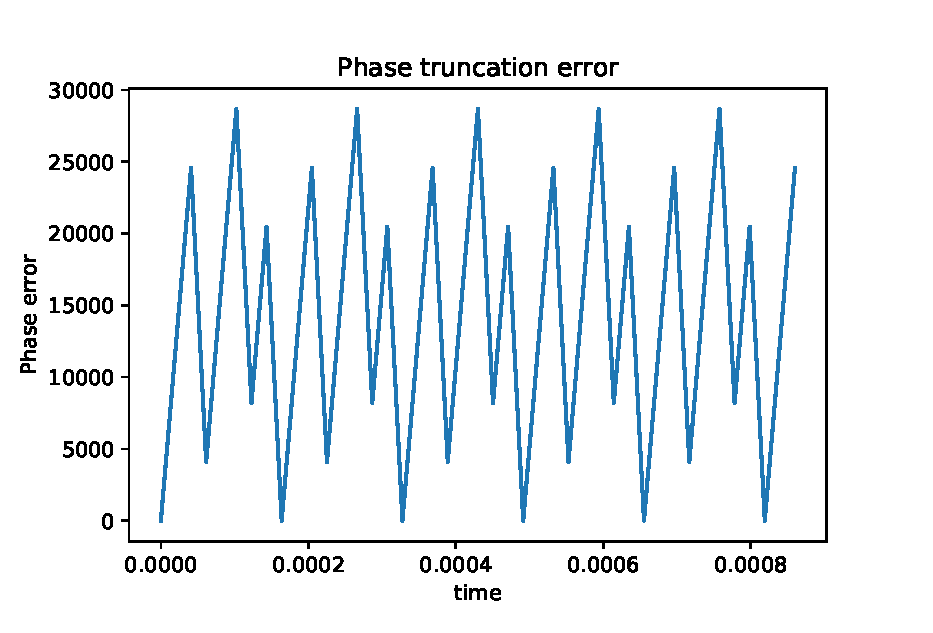
\includegraphics[width=0.85\columnwidth]{TeX_files/phase_truncation_error.eps}
	\caption{Periodicità dell'errore di troncamento di fase corrispondente alla $\code{FTW}=63565$, con $\code{N}=32$ e $\code{M}=17$.}
\end{figure}

In generale quindi l'errore introdotto dalla DDS dipende da $M$ e $N$ ed è diverso per ogni
scelta della \code{FTW}. Si veda \cite{analogdevicessec4} oppure \cite{exactspurs} per una trattazione
più dettagliata della distribuzione e ampiezza delle frequenze spurie nel segnale,
omessa in quanto complessa dal punto di vista matematico.

La riduzione di SNR dovuta alla DDS è stata calcolata, attraverso le simulazioni,
per ogni possibile valore del \textit{note number} ed è riportata in \cref{fig:confronto}.

Per $\code{N}=32$ l'SNR decresce fino a circa $\SI{47}{\decibel}$ per alcune
frequency tuning words. Usando una precisione maggiore per il registro di fase
si riesce ad ottenere un SNR al minimo di \SI{58.8}{\decibel}, molto vicino a quello di sola quantizzazione.


\begin{figure}[H]
    \begin{minipage}{0.59\columnwidth}
            \centering
            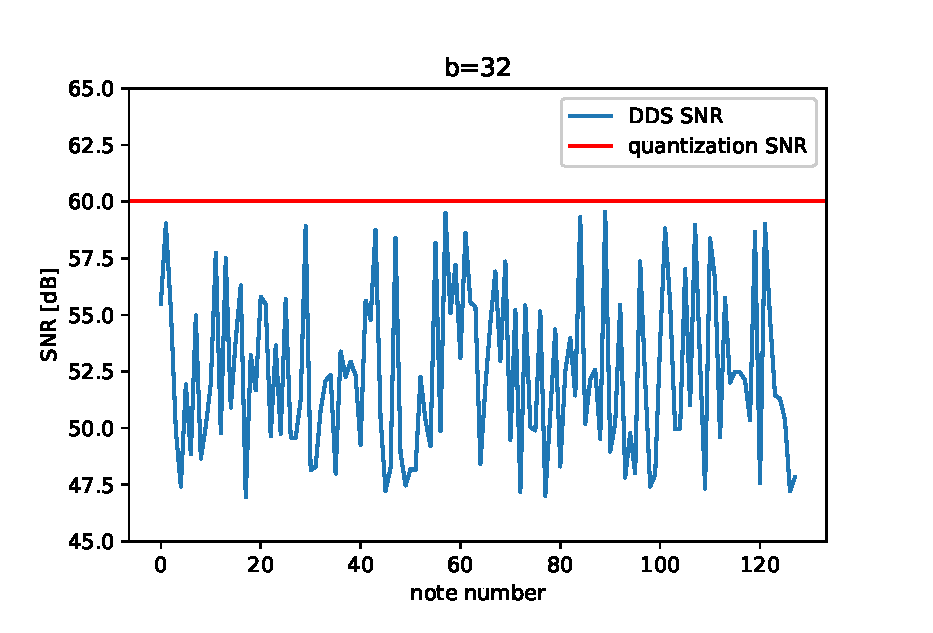
\includegraphics[width=1.0\columnwidth]{TeX_files/dds_snr_32.eps} % first figure itself
        \end{minipage}\hfill
    \begin{minipage}{0.59\columnwidth}
            \centering
            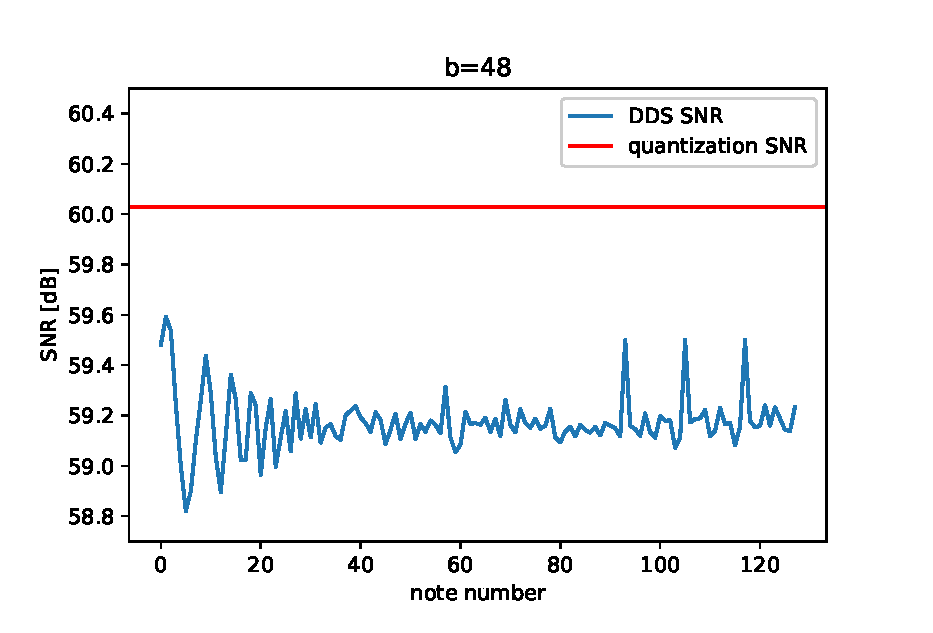
\includegraphics[width=1.0\columnwidth]{TeX_files/dds_snr_48.eps} % second figure itself
    \end{minipage}
    \caption{Confronto dell'SNR dovuto alla DDS con due grandezze diverse del registro di fase.}
    \label{fig:confronto}
\end{figure}

\section{Considerazioni finali}
Il sintetizzatore progettato, sebbene funzionante, presenta performance
di SNR non ottimali, dovute alle limitazioni intriseche della pulse-width 
modulation.
La PWM infatti limita il numero di bit di risoluzione del campionatore da un lato
e la frequenza massima rappresentabile dall'altro.
Sarebbe possibile bypassare l'uscita audio monofonica della scheda
e utilizzare un DAC esterno, connesso attraverso le porte PMOD, 
per fornire una qualità audio migliore.
Due esempi sono i componenti PMOD I2S2 e il PMOD AMP2 della Digilent.

La polifonia, essendo implementata con un semplice sommatore in fase 
di mixing, è soggetta ad overflow quando la somma dei campioni supera
la precisione permessa dai \code{b} bits di quantizzazione.
In campo audio questo fenomento viene detto \textit{clipping}.
Di fatto, essendo l'ampiezza del segnale campionato pari a poco meno
della metà del valore massimo rappresentabile, la polifonia è limitata
a due voci, oltre le quali il segnale presenta una degradazione
notevole.

Far rientrare il range del segnale nei limiti con un divisore risolverebbe
il clipping ma degraderebbe la qualità del segnale e causerebbe
sbalzi di volume udibili nel passaggio da una singola nota  a più note
suonate contemporaneamente.

Tecniche più avanzate di compressione dinamica del segnale 
sono molto complesse e al di fuori dello scopo di questa tesi.  

I messaggi MIDI contengono anche l'informazione relativa alla forza
di pressione della nota, detta velocity, come descritto nel \cref{chap:midi}.
Si potrebbe estendere il sintetizzatore per rispettare questa informazione
in due modi differenti:
\begin{itemize}
  \item Si stabiliscono dei range di velocity meno granulari  e per ognuno
        di questi si accede a una rom diversa creata impostando una diversa 
        ampiezza alla forma d'onda
  \item Si stabiliscono sempre dei range di velocity, ma lo scaling dei
        campioni avviene con un divisore
\end{itemize}
Il primo metodo produrrebbe risultati più precisi numericamente ma al
prezzo di una notevole quantità di memoria in più, mentre il secondo
otterrebbe una qualità peggiore ma con un'occupazione minore delle
risorse del FPGA.

Il sintetizzatore è stato operato attraverso un 
computer per il testing, ma sarebbe possibile connettere la scheda
direttamente utilizzando una porta PMOD generica e un circuito esterno
(anche su breadboard) a cui connettere il jack MIDI.
